%% TITOLO
\section{Sistemi Autonomi}
\label{sec:Sistemi Autonomi}

Nel capitolo precedente, attraverso la composizione e gli studi di Agostino Di Scipio, 
abbiamo potuto osservare che cosa si intende, e come viene organizzato, 
un sistema con non linearità provenienti dal mondo fisico; aperto al suo ambiente esterno 
che diviene in questo caso lo spazio stesso della performance.
Sempre in riferimento alla cibernetica di secondo ordine,
abbiamo già parlato del fatto che nessun sistema è separabile e 
isolabile da un suo ambiente circostante, 
ma abbiamo osservato anche come il concetto di spazio di un sistema sia 
qualcosa di molto complesso, poiché il concetto stesso di "complessità"
sta a significare in un sistema che questo sia composto da una rete d'interazioni dinamiche, 
ma che il comportamento dell'insieme potrebbe non essere prevedibile in base al comportamento 
dei diversi componenti tipicamente in relazione fra loro.
Mentre, nel caso di Agostino Di Scipio, lo spazio del sistema che ne contiene le sue relazioni 
è costituito principalmente dal mondo fisico, 
in questo capitolo osserveremo come, per lo spazio di un sistema, 
si possa intendere anche uno spazio latente, 
che traccia le sue relazioni tra le parti in uno spazio virtuale interamente programmato nel software. 
In questo caso, l'ambiente digitale che racchiude il sistema all'interno e le sue relazioni 
tra gli agenti è interamente costituito solo dal DSP, 
inclusi i metodi per la generazione delle relative non linearità.
Ho voluto approfondire questo metodo attraverso il lavoro compositivo e gli studi di Dario Sanfilippo, 
specialista di sistemi di feedback, esecutore e compositore. 
I suoi lavori riguardano principi di autopoiesi, evolvibilità e costruttivismo radicale nella progettazione 
di reti di feedback audio complesse. \\
La modalità con cui andrò a discutere in questo capitolo la composizione di questi
sistemi autonomi, appartenenti anche questi alla più vasta categoria dei CASes (Complex Adaptive Systems), 
è ponendo un focus su un particolare lavoro di Dario Sanfilippo, Order From Noise \textit{(Homage to Heinz Von Foerster)}. \\
Order From Noise \textit{(Homage to Heinz Von Foerster)} è un progetto che implementa uno 
dei primi prototipi di Dario Sanfilippo basati sull'idea dell'\textit{adattattività dinamica}. 
Questo lavoro del compositore si basa sull'idea che i sistemi adattivi complessi, 
che sono emergenti per definizione, siano essenziali per raggiungere innovazioni formali, 
performative e tecniche, nel contesto della performance in Live Electronics e nella composizione musicale in generale. 
\footcite{sanfilippo_time-variant_2018}
I CASes si dicono adattivi quando sono composti da una rete dinamica 
di interazioni dove i singoli agenti interconnessi fra loro, interagendo individualmente
o collettivamente, possono cambiare il loro stato in risposta a variazioni nell'ambiente o
degli altri agenti connessi. 
Questo tipo di relazioni nel sistema è comune sia nell'opera di Agostino Di Scipio,
in cui abbiamo visto precedentemente come lo stato dei singoli agenti nel sistema 
cambi al variare delle condizioni nell'ambiente circostante portando a
cambiamenti di stato globali del sistema, che nel lavoro di Dario Sanfilippo.
Altro importante aspetto in comune qui con l'opera di Agostino Di Scipio,
è il tipo di rapporto che ha l'uomo con la macchina, che viene respinto nella visione in cui è il primo
ad essere totalmente a controllo del secondo, per essere sostituito da un concetto 
d'interazione Uomo-Macchina-Ambiente, chiamato da Dario Sanfilippo Ibridazione: 
una condizione in cui umano e macchina cooperano per far emergere la performance. 
Nel caso delle opere di Dario Sanfilippo, tuttavia, l'estetica dei suoi lavori è interamente subordinata
al disegno del sistema stesso, che di volta in volta, emerge da fenomeni musicali che sono il risultato
del tipo d'interazione che viene a crearsi fra il performer e il disegno del sistema che si era reso necessario
in partenza. \\
In alcuni casi, questa idea viene portata alle sue estreme conseguenze con opere in cui la macchina è l'unica 
ente che esegue, come accade per il brano presentato qui.

\begin{center}
    \vspace{0.5cm}
    \textit{Order from noise (2017) is based on a time-variant feedback delay network containing a 
    set of entangled nonlinear processing algorithms for audio and information signals. 
    The work is an example of autonomous self-performing system and it is realised by
    feeding the network with one millisecond of background noise from the performance
    environment. The initial recirculating noise impulse is what entirely determines the
    formal evolutions of the system which have substantially different long-term developments 
    for each different noise impulse. An approach to present the work live is that
    of reinitialising the system a number of times for a period of about three-five minutes
    to show its sensitivity to initial conditions and the long-term divergence between the
    formal structures.}\footcite{sanfilippo_time-variant_2018}
    \vspace{0.5cm}
\end{center}

Rispetto al sistema discusso nel capitolo precedente, 
come già accennato c'è una sostanziale differenza nel concetto di spazio
o ambiente del sistema. 
Come appena detto, Order From Noise è basato su una \textit{feedback delay network} 
tempo-variante, vuole dire che ci ritroviamo di fronte ad un un sistema il cui
funzionamento cambia nel tempo, a differenza dei sistemi tempo-invarianti
dove seppur l'output del sistema può cambiare nel tempo, 
il loro funzionamento e l'ambiente che contiene il sistema rimane inalterato.
In parole semplici lo spazio del sistema in Order From Noise può variare nel tempo,
rendendo imprevedibile il suo funzionamento a partire da una determinata condizione 
iniziale.
Per questo motivo il performer non avrà un grande margine di prevedibilità 
nel comportamento del sistema a differenza dei sistemi tempo-varianti,
ma saprà che per le stesse condizioni iniziali, il sistema qui totalmente
deterministico, riporterà sempre le stesse evoluzioni formali.
Proprio come nei Sistemi Caotici emersi dalla Teoria del Caos introdotti all'inizio di questa tesi,
che seppur governati da leggi deterministiche, 
sono in grado di esibire un'empirica casualità nell'evoluzione delle variabili dinamiche. \\

\subsection{Audio Information Processing}
\label{sec:Audio Information Processing}
Come già accennato nello scorso capitolo, l'\textit{Audio Information Processing};
ovvero la capacità di un sistema di elaborare le informazioni
tremite la \textit{feature extraction}, è un dato fondamentale nella creazione 
di un CAS, che ne determina le sue capacità "congitive" e di auto-osservazione
rispetto all'ambiente. 
L'uso creativo dei CASes in Musica,
e la loro stretta connessione con l'informazione,
ha favorito lo sviluppo di techniche algoritmiche per l'\textit{Audio Information Processing} 
e l'analisi di comportamenti, sia ad alto e basso livello.

\begin{center}
    \vspace{0.5cm}
    \textit{The low-level algorithms provide a continuous measure of the features and can operate
with short analysis frames. The high-level algorithms, on the other hand, are original designs informed both perceptually
and by complexity theory for the analysis of musically meaningful information, both in short sounds or articulated
streams with long-term nontrivial variations.}\footcite{sanfilippo_time-domain_2021}
\vspace{0.5cm}
\end{center}

Alcuni primi esempi storici,
sono ad esempio le performance in Live Electronics di Gordon Mumma, 
come“Diastasis, as in Beer” (1966), e "Hornpipe" (1967), 
dove vengono implementate techniche di amplitude following utilizzate 
poi per pilotare parametri nelle unità di generazione del suono.\footcite{sanfilippo_time-domain_2021}
Arrivando fino ai sistemi di Agostino Di Scipio, che nello studio del suo
Feedback Study ci ha dato modo di approfondire e scoprire
tutti quei meccanismi e tutte quelle particolari funzioni che hanno la responsabilità
di generare segnali di controllo nei suoi sistemi. \\
Dario Sanfilippo ha discusso in più articoli l'utilizzo dell'\textit{Information Processing} 
nei CASes, sia in senso generale\footcite{sanfilippo_time-domain_2021}, 
parlando di implementazioni più tipiche come: 
centroide spettrale, rumorosità, diffusione spettrale a basso livello, eterogeneità e
complessità per l'alto livello.
Che come in questo caso nell'utilizzo specifico di queste tecniche 
in un suo sistema:

\begin{center}
    \vspace{0.5cm}
    \textit{These signals, often based on
    their perceptual characteristics and their relationship with the domains of the variables
    in the processing units, are mapped to certain ranges and then used to control the state
    of the components in a large network. (See Di Scipio (2003) for a detailed discussion
    on this method). Using infrasonic signals to pilot these variables is highly desirable if
    not necessary, for high-rate, sudden changes in the DSP parameters would produce an
    output with a continuously large and homogeneous spectral band, so it would not be
    possible to perceive the state variations in the long-term.
    The information and audio processing algorithms implemented, the specific con-
    nections between the control signals and the variables, the linear and nonlinear map-
    ping strategies used as well as the network topologies, all these elements determine the
    infrastructure of a system. In a large network, these elements can already provide a high
    number of configurations and an even larger number of possible states that a system
    can reach. That, theoretically, could be considered as something that guarantees a good
    variety and complexity in the long-term behaviour of a system, albeit the practical case
    tends to be much different from the ideal scenario.}\footcite{sanfilippo_time-variant_2018}
    \vspace{0.5cm}
\end{center}

Nel suo articolo su Order From Noise, Sanfilippo discute tutte le unità utilizzate
nel suo sistema e il loro ruolo all'interno della rete.
Partendo dalla descrizione di queste nell'articolo, tratterò ora una parte più operativa 
implementando queste tecniche nel linguaggio di programmazione FAUST (Grame), 
con un particolare Focus a tutte quelle \textit{feature extraction}
che nell'implementazione della rete permettono al sistema 
(nonostante questo sia chiuso rispetto all'ambiente esterno) 
di mantenersi in uno stato "emergente" manifestando comportamenti nuovi,
e di "stabilità", rimanendo sempre in dei range controllati tramite feedback positivi e negativi.\\
La rete di Order From Noise ha sei nodi, ognuno dei quali contiene due unità in cascata, 
contenenti i seguenti algoritmi di elaborazione audio: 
\textit{asynchronous granulation, recursive comb filtering, variable high-pass/low-pass filtering, pulse-width mod-
ulation (PWM), resampling and 16th-order feedback delay network (FDN) processing.}

\begin{center}
    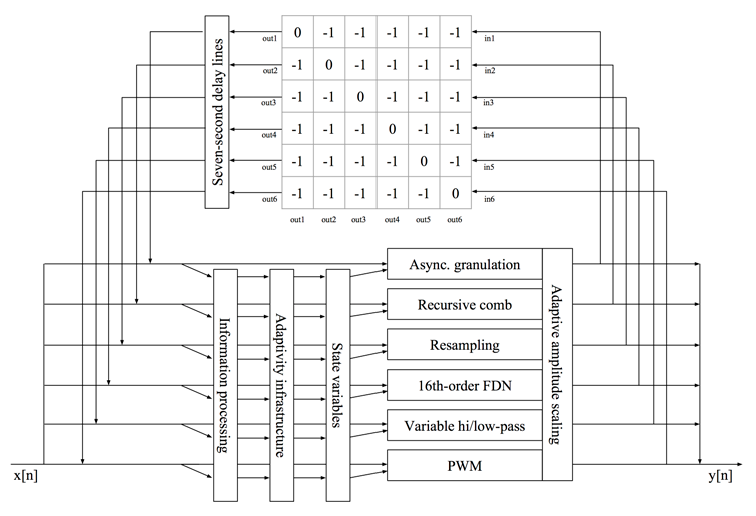
\includegraphics[width=12cm]{figures/OFNnetwork.pdf} \\
    {Schema della rete di Order From Noise} \\ 
    \end{center}

A parte le unità di elaborazione del suono,
in questo sistema,l'\textit{Information Processing} utilizzato per generare i 
segnali di controllo è diverso
dalle implementazioni tipiche riportate precedentemente nel corso di questa tesi;
piuttosto che calcolare \textit{feature extraction} come l'RMS, la diffusione spettale, ecc. 
Dario Sanfilippo utilizza in questo sistema una sorta di Low Frequency Oscillator
non lineare dipendente dal segnale in ingresso.
Questo comportamento viene ottenuto utilizzando un filtro Lowpass per far 
passare solo le componenti energetiche di un segnale sotto la soglia di 1Hz,
come ad esempio segnali a 0,01Hz, il segnale risultante viene poi processato
tramite normalizzazione dinamica per essere riportato ad una soglia in ampiezza
in un range fra [-1; 1],
viene elevato a una potenza relativamente grande per forzarlo intorno a 0,
ed infine utilizzato per pilotare la frequenza di un fasore.\\


- algoritmo


Lookahead Limiters per la stabilità delle Feedback Network:
In Order From Noise Dario Sanfilippo utilizza un unità per raggiungere la stabilità
globale della rete chiamata Lookahead Limiter.

<< My original design was based on two side-chained amplitude curves: 
a fast one for attack transients and one for sustained sounds, which had 
to be slow enough as to avoid intermodulation distortion. The fast curve 
was based on peak envelope estimation (see below), while the slow one was based on 
RMS to have a smooth behaviour. The curves were in a master-slave mode so that 
the effect of the fast curve would decrease with regard to the growth of the slow curve: 
that was necessary to avoid that the processed signal would be scaled down twice by both curves. 
Despite the algorithm produced good results, it needed some empirical calibrations 
and it also involved a rather large number of objects in Pure Data which would considerably load the CPU. 
Besides, I was using some objects from PD-extended and I already had in mind to migrate to Pure Data Vanilla.
A simplified design was based on only one amplitude curve calculated with a long-decay peak envelope (10 seconds). 
A peak envelope checks whether the input is greater than the output and, if that condition is true, 
it updates the peak with the new value from the input signal. 
Otherwise, the current peak decreases following an exponential curve and reaches a certain 
attenuation after a desired time which, in my specific case, is of ~60dBs. 
This would allow detecting fast attack transient and, at the same time, 
the long decay would create a smooth curve for the sustained and slow sounds. >>
https://www.dariosanfilippo.com/blog/2017/lookahead-limiting-in-pure-data/

This was a good compromise for my systems, although such a long decay is not always desirable: occasionally, 
that would create silences after high-amplitude impulses for the attenuating curve 
would decrease very slowly and the input signal would be scaled down even if below the limiting threshold.